
%(BEGIN_QUESTION)
% Copyright 2015, Tony R. Kuphaldt, released under the Creative Commons Attribution License (v 1.0)
% This means you may do almost anything with this work of mine, so long as you give me proper credit

A technician needs to write a PLC program to control a water pump driven by an electric motor.  This water pump will be manually started and stopped by pushbutton switches, and shut down automatically by any one of several ``permissive'' switches.  The operating statuses of these switches are listed here:

\begin{itemize}
\item{} {\bf Start pushbutton} (normally-open): open when unpressed, closed when pressed
\item{} {\bf Stop pushbutton} (normally-open): open when unpressed, closed when pressed
\item{} {\bf Low water level} (normally-closed): closed when level is low, open when level is adequate
\item{} {\bf Low oil pressure} (normally-open): open when pressure is low, closed when pressure is adequate
\item{} {\bf High vibration} (normally-closed): closed when still, open when vibrating
\item{} {\bf Water leak detector} (normally-open): open when dry, closed when wet (leak detected)
\end{itemize}

The technician's first attempt is shown here, but it contains a serious error.  Identify and correct this error:

$$\includegraphics[width=15.5cm]{i02658x01.eps}$$

\underbar{file i02658}
%(END_QUESTION)





%(BEGIN_ANSWER)

The {\tt Stop\_PB} contact instruction should be drawn as normally-closed rather than normally-open as shown in the technician's first draft of the PLC program.  The program is designed to shut down the motor when that pushbutton is pressed (i.e. the {\tt Stop\_PB} contact instruction becomes uncolored (i.e. fails to ``conduct'' virtual power).  We have been told that the real-world Stop pushbutton switch is NO, which means its contact closes when pressed.  This means pressing the Stop pushbutton causes that bit to be 1, which necessitates an NC contact instruction so that it will un-color under that condition.

%(END_ANSWER)





%(BEGIN_NOTES)


%INDEX% PLC, diagnosing programming error
%INDEX% PLC, relating I/O status to virtual elements (troubleshooting)
%INDEX% PLC, troubleshooting: motor start/stop control circuit

%(END_NOTES)


